\section {EVALUATION} \label{sec:evaluation}

We carefully evaluated our integrations in several qualitative and quantitative areas. For each of our integration interfaces (CLI, gRPC, and REST API), we ran the integration against a single test image from Wikipedia and measured the amount of time from passing the image to Tika (and Tensorflow) to the return of a classification result from the API. All single-image tests were run on an Ubuntu 14.04 LTS Docker container running on MacBook Pro 2013 model (2.8GhZ Core i7 and SSD storage) for test images of size 1024x768 pixels. The slowest integration by far was the CLI integration which took 3 seconds to return a result, the fastest integration was the REST integration at 253ms, about twice as fast as the gRPC integration at 598ms. However, REST uses more bandwidth due to additional metadata introduced by HTTP headers in the packets, compared to gRPC which does not require additional HTTP headers.

The REST integration benefitted from a pre-loaded ImageNet/Inception model, along with lightweight dependencies and low overhead. The gRPC interface, while fast, suffered qualitatively from relying on conflicting HTTP client library transitive dependencies, making it difficult to integrate with some functionality from older HTTP clients and reducing the number of platforms it successfully deploys on. Though slow, the CLI has the advantage of not requiring both a client and server, eliminating an additional point of failure in a distributed setting. However, its sluggishness can be attributed to the extra process created per invocation and the I/O for each call, since the model file is loaded and unloaded for each process. In addition, the ImageNet/Inception model is approximately 200MB in size, so there is 200MB of additional I/O per parse call.

While we did explore JNI integrations in our interface, we didn't implement a full solution as we would have had to produce JNI glue code for all platforms and additional utilities such as Google's ProtoBuffers -- a dependency required by Tensorflow -- would have to be integrated with the JNI because ProtoBuffers is required for deserializing models such as ImageNet/Inception\cite{javacpp-240}. The results  were encouraging both qualitatively and quantitatively; using the REST interface, we were able to index the entire 1.4 million image Memex weapons dataset in a little over four days.

\begin{figure}
	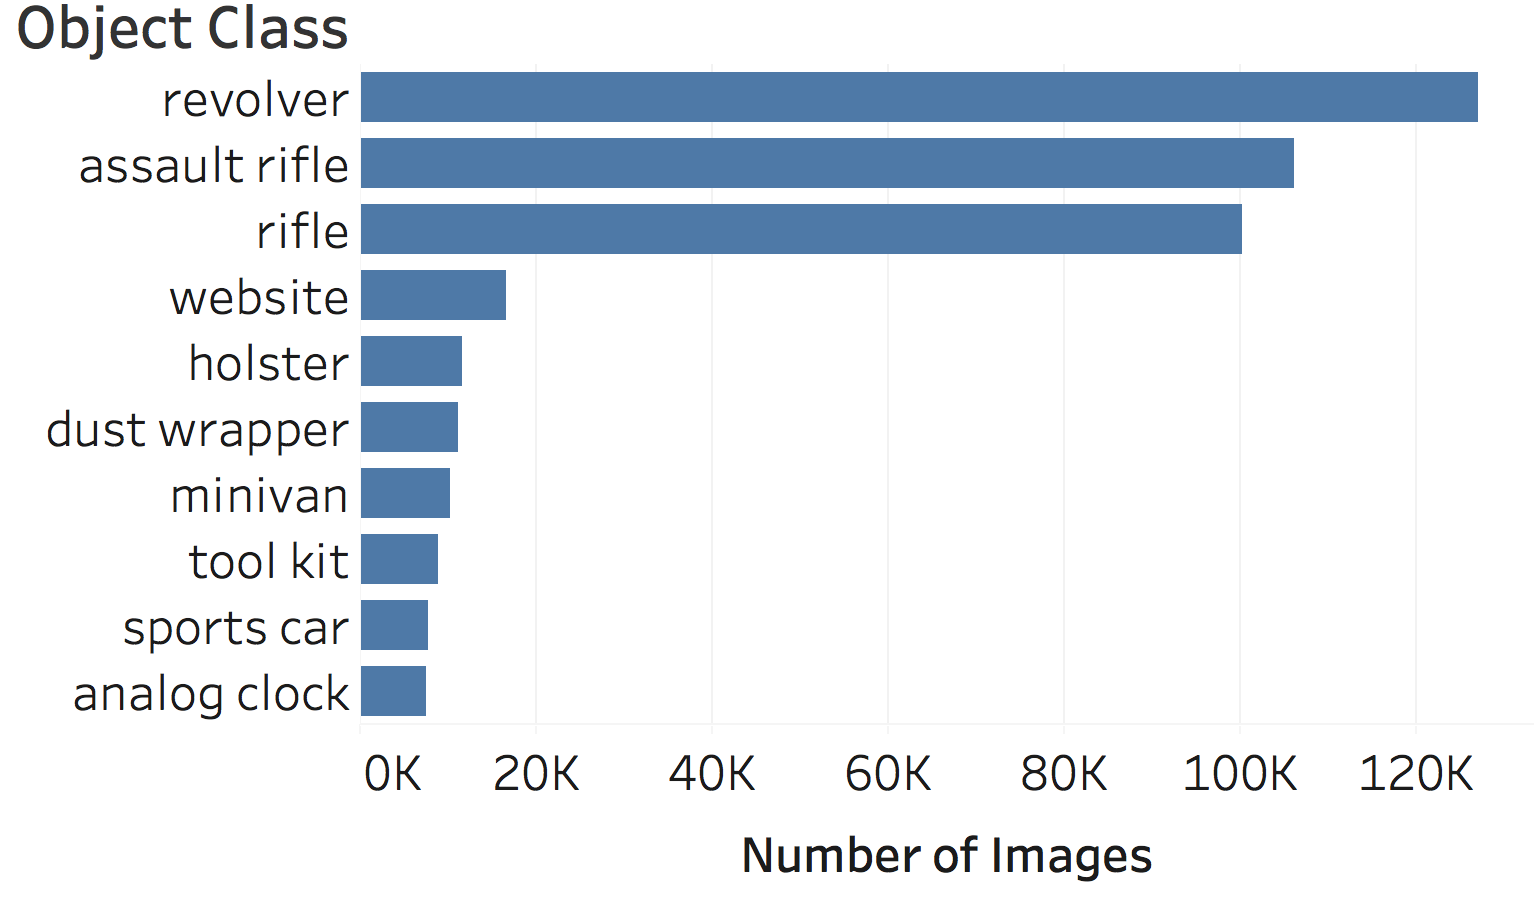
\includegraphics[width=\columnwidth]{top10classes2}
	\caption{Top 10 image classes found in the dataset. As more labeled weapon images become available, we will be able to train a custom classifier to classify weapons with more granularity.}
	\label{fig:top10ImgClass}
\end{figure}


In addition to qualitative and quantitative evaluation of our integration techniques, we also evaluate the results of our image classification with respect to automatic processing of the Memex weapons dataset.  We used the \textit{Inception v3} image classification model in our experiments \cite{SzegedyVISW15}. This model was trained on the 2012 ImageNet dataset, which contains 1000 classes of objects\cite{ILSVRC15}. The ten most frequently occurring classes and their frequencies are shown in Figure \ref{fig:top10ImgClass}. Since the crawlers were focused on retrieving web pages and linked images related to weapons classifieds, the top classes in our dataset were found to be \textit{revolver} and \textit{rifle}. Automatically identifying \textit{rifle} in this dataset was a promising result, as it gave investigators leads in discerning whether these were long guns, which have been increasingly used in weapons-related deaths over the past decade. Also promising was the second most fequenty occurring class, \textit{assault rifle}, which provides investigative leads into potentially automatic weapons in the dataset.

We cross-validated the predictions using a subset of human-labeled images, and the results are shown in Figure \ref{fig:uk-hack-eval}. The \textit{top k} for $k=1,3,5,7$ considers a prediction as correct if the human annotated label is among the set of top $k$  predicted labels. We observed that the \textit{top 1} accuracy for the \textit{revolver} class is considerably lower. Manual inspection of labeled images and prediction errors revealed that, due to revolvers being smaller, they are often surrounded by holders and toolkits. The \textit{Inception} model often treated these larger surrounding objects as the predominant label rather than the \textit{revolver} label. Hence, the error counts are reduced when $k$ is increased. Going forward, our team is interested in more granular distinctions. For instance, the model doesn't discern between \textit{rifles} and \textit{shotguns} - all of these weapons are mapped to the \textit{rifles} label in the current \textit{Inception} model. 

%//TODO: Describe more if space permits
\begin{figure}
	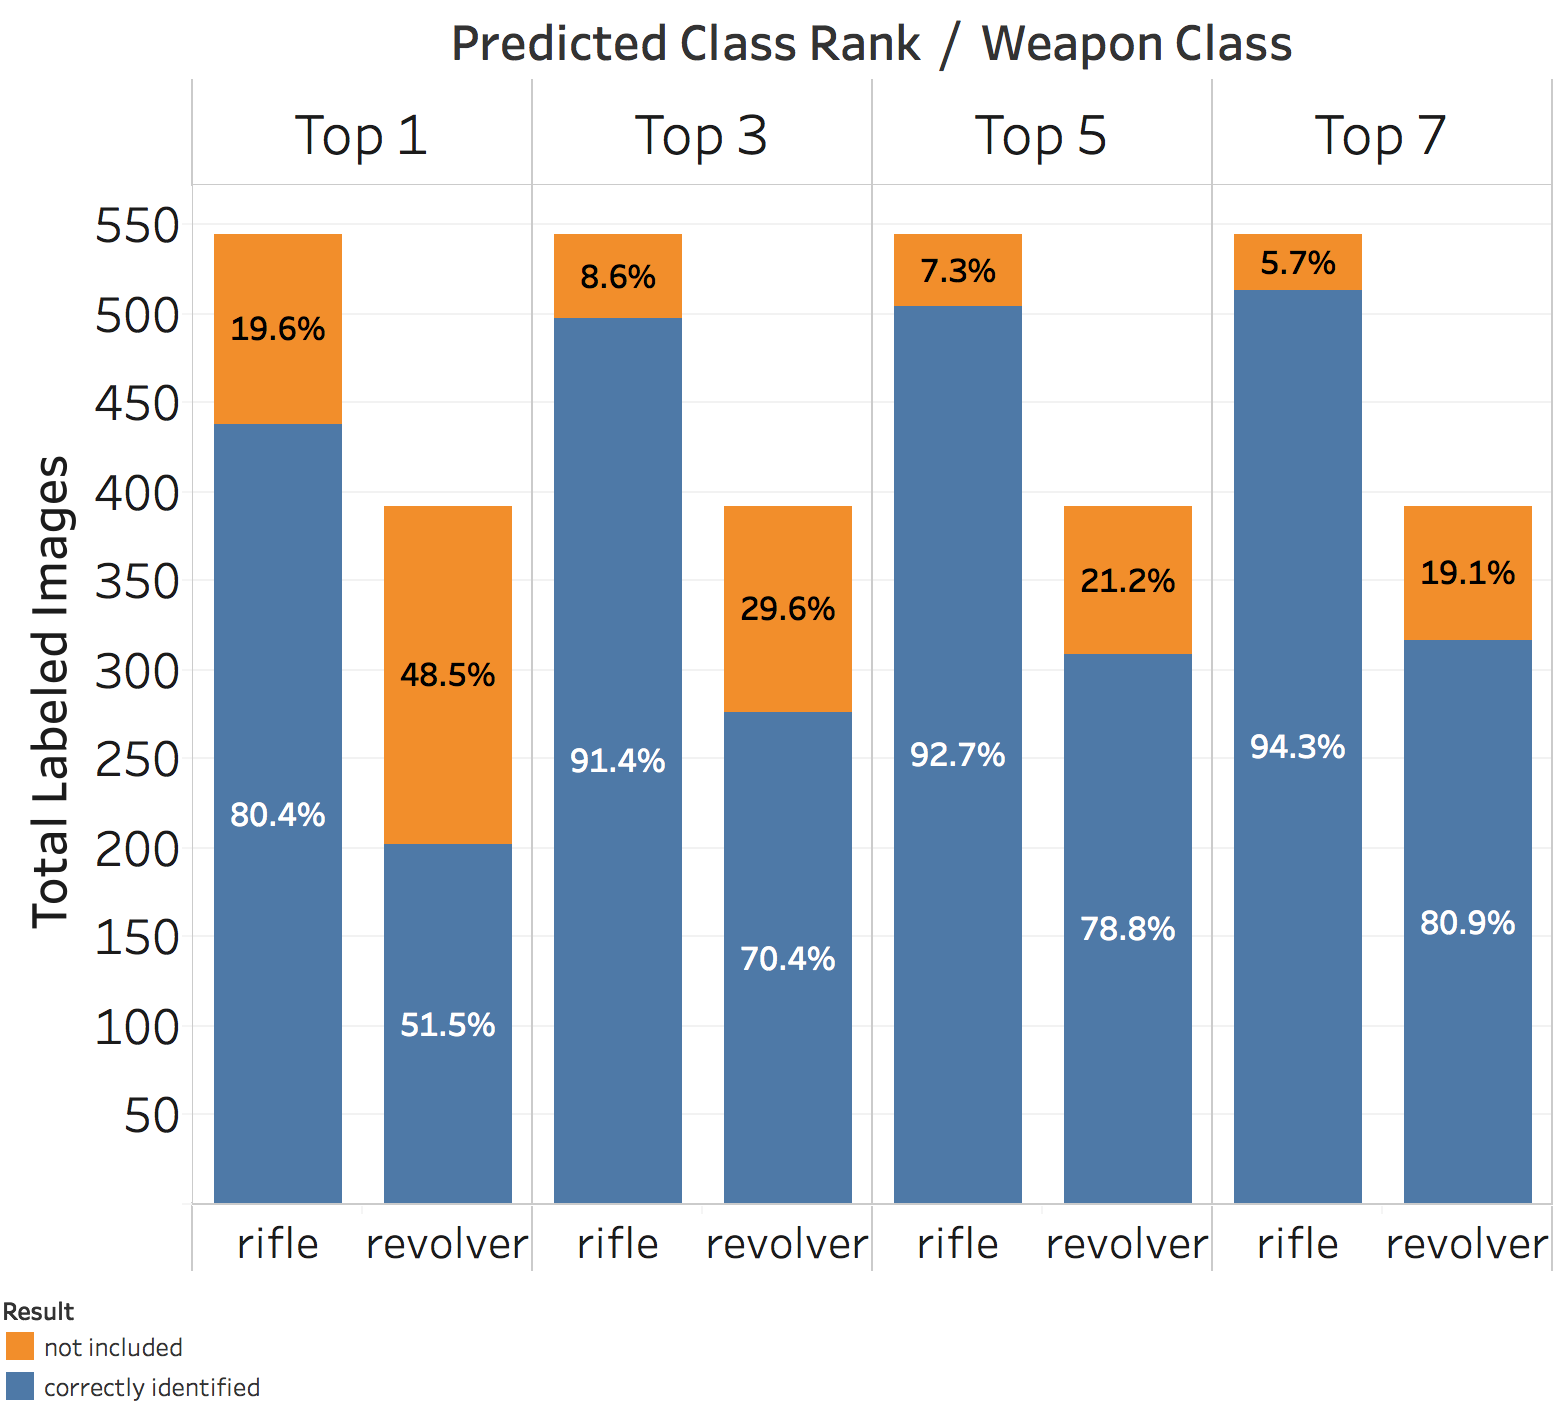
\includegraphics[width=\columnwidth]{uk-hack-evaluation3}
	\caption{Manual cross validation of results for the two weapon types: `revolver' and `rifle.' The weapon object should be the top class for all labeled images, however these results demonstrate that the model occassionally identified background objects as primary.}
	\label{fig:uk-hack-eval}
\end{figure}

